\documentclass[a4paper,12pt]{article}
\usepackage{HomeWorkTemplate}
\usepackage{circuitikz}
\usepackage[shortlabels]{enumitem}
\usepackage{hyperref}
\usepackage{tikz}
\usepackage{amsmath}
\usepackage{amssymb}
\usepackage{tcolorbox}
\usepackage{xepersian}
\usepackage{graphicx}
\usepackage{tikz}
\settextfont{XB Niloofar}
\usetikzlibrary{arrows,automata}
\usetikzlibrary{circuits.logic.US}
\usepackage{changepage}
\newcounter{problemcounter}
\setcounter{problemcounter}{1}
\newcommand{\problem}[1]
{
	\subsection*{
		بخش
		\arabic{problemcounter} 
		\stepcounter{problemcounter}
		#1
	}
}


\begin{document}
\handout
{ساختار کامپیوتر و میکروپروسسر}
{دکتر باقری شورکی}
{نیم‌سال اول 1399\lr{-}1400}
{اطلاعیه}
{صدرا صبوری هلستانی}
{97101972}
 {توضیحات پروژه اول - طراحی میکروپروفسور}
\problem{}
دستگاهی که در ابتدا طراحی آن هستیم دستگاهی است که وظیفه اجرای دستورات برنامه (به عنوان ورودی) به صورت $Real-Time$  و ذخیره تاثیرات آن روی حافظه برای استفاده کننده از آن را فراهم می سازد، با توجه به نظریه ماشین های اتوماتا طراحی چنین ماشین محاسبی در حالت کلی یک مسئله تصمیم ناپذیر ولی تشخیص پذیر است به این منظور قطعه کدی که روح اصلی برنامه را اجرا خواهد کرد باید توانایی رفتار با خانه های حافظه به همان شکلی که سیستم اصلی با کد اصلی برنامه رفتار میکند را داشته باشد-یعنی 3 مرحله $Fetch, Decode, Execute$ ولی این بار به صورت نرم افزاری-.
\\
\\
مطابق عملکرد نسخه اول همین محصول در دنیای واقعی، عملکرد کلی این دستگاه به این شکل است که ابتدا با فشردن دکمه $ADDRESS$ توسط کاربر دستگاه در وضعیت نمایش اطلاعات خانه های حافظه را به خود بگیرد و با وارد کردن خانه مورد نظر حافظه توسط کاربر، اطلاعات خانه مشخص شده نمایش داده شود، ضمنا بهتر است زمانی که تعداد ارقام وارد شده توسط کاربر از تعداد مشخصی بیشتر شد، ارقام نشان دهنده آدرس از سمت دیگر خارج شوند، همچنین بهتر است برای \underline{جلو گیری از اختلاط کد اصلی و حافظه مورد نیاز برنامه اصلی با برنامه کاربر} ، آدرس را از مکان مشخصی، مثلا $1000H$ آغاز کنیم (برای حالتی که کد برنامه را رد $ROM$ می ریزیم و کد دیتا در $RAM$ است این ملاحظه نیاز نیست).
\\
\\
در گام بعدی، بعد از مشخص شدن مکانی که باید در آن داده را بنویسیم، با فشردن $Data$ میتوانیم داده مورد نظر را در مکان آدرس مورد نظر بنویسیم (این داده میتواند $Op Code$ مربوط به دستورت یا $Operand$ مربوط به دستورات باشد) و نیز برای ذخیره شدن آن از دکمه های + یا – استفاده بکنیم که یک خانه به بالا یا پایین برویم و محتویات آن خانه ها را عوض کنیم.
\\
\\
نمای اولیه طراحی شده برای این پروژه به صورت زیر است:

یکی از معایب پروتئوس این است که\underline{کیبرد مناسب به اندازه 8 در 8 ندارد} و به جای آن از keypad 4 در 4 استفاده کردیم و با $decompose$ کردن مدل و عوض کردن نام کلیدها آنان را به دلخواه خود در آوردیم، اما مشکل اینجاست که برای وارد کردن ورودی ها که در مبنای 16 است تعداد ارقام است این مشکل در قسمت آدرس با دکمه های + و – قابل حل است ولی برای قسمت داده میتوان هم محدودیت ورودی اعداد ایجاد کرد و هم میتوان عدد ورودی توسط کاربر را به صورت در مبنای 10 تعریف کرد و بدین صورت میتوان از 0 تا 255 را در 4 سون سگمنت باقی مانده نمایش داد و در آخر باقی مانده تقسیم عدد ورودی توسط کاربر را بر 256 به عنوان عدد ورودی مورد استفاده قرار می گیرد.
\\
\\
اجزای اصلی مدار مطابق خواست سوال طراحی شده اند 2 دیکودر یکی برای تبدیل اعداد به معادل سگمنت های 7سگمنت و دیگری برای مشخص کردن اینکه الآن کدام یک از 7 سگمنت ها می بایست روشن شود مورد استفاده قرار میگیرد، این کار باعث میشود که بتوان با تنها استفاده از یکی از پورت های آی سی 8051 کل فرآیند نمایش را کنترل کرد که می دانیم بسیار ارزشمند است، زیرا احتمالا به زودی با \underline{مشکل کمبود پورت} مواجه خواهیم شد.
\begin{figure}[htbp]
\centerline{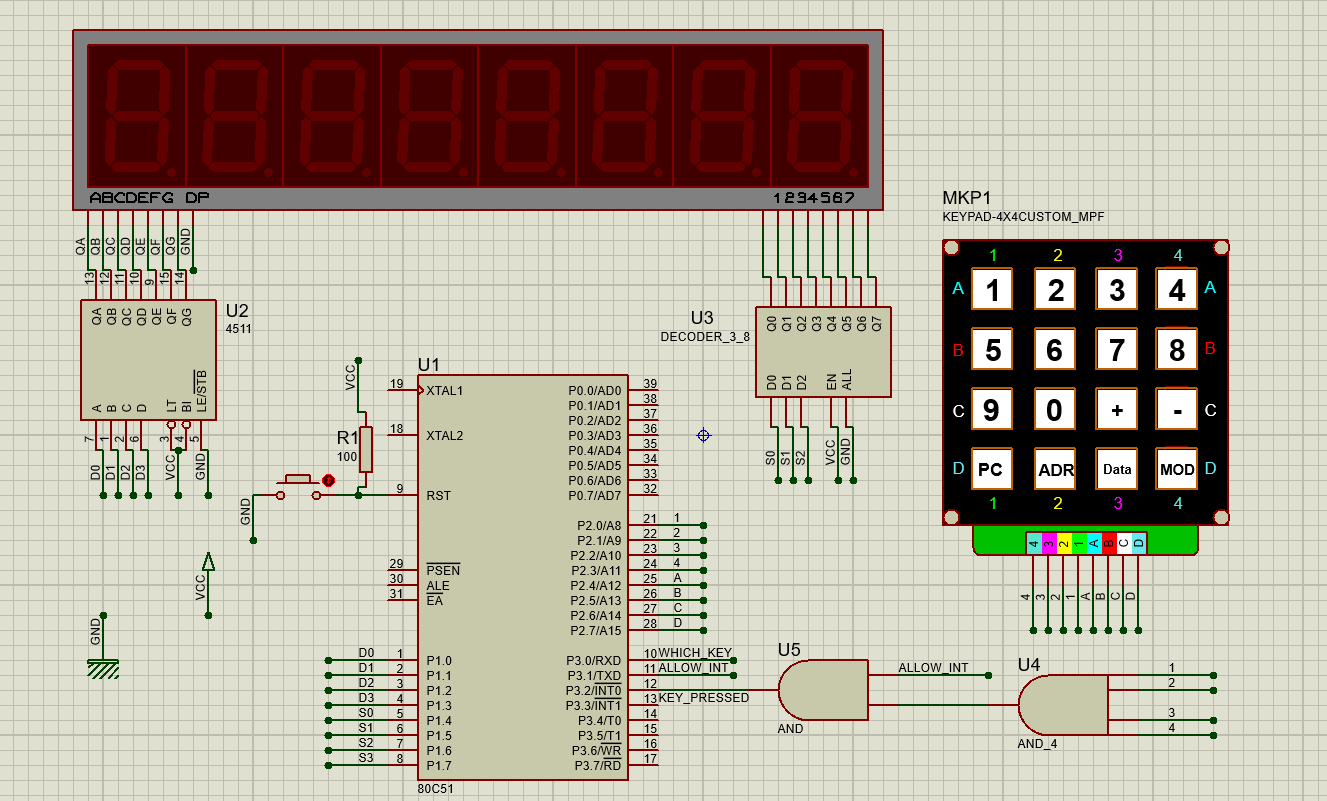
\includegraphics[width=6.625in, height=4in]{../Others/MAIN_CIRCUIT.PNG}}
\caption{نمایی از طراحی اولیه مدار}
\label{fig}
\end{figure}
فرآیند تشخیص کلید زده شده هم مانند آزمایش 7 ام آزمایشگاه این درس با کلیک شدن حداقل یکی از کلید ها $Interrupt$ مربوط به کلید فعال می شود و $CPU$ مشغول دریافت ورودی از کاربر می شود.
\\
\\
بعد از اتمام این مراحل بهتر است فضایی را برای دیتایی که باید برای نمایش به روی 7 سگمنت ها استفاده بشوند را در محلی ذخیره کنیم (هر رقم معادل یک بایت است و با در نظر گرفتن 8 بایت برای نمایش این اعداد می توان پیوسته این اعداد را نمایش داد و از طریق برنامه تنها محتویات این خانه ها را عوض کنیم که این موضوع باعث عوض شدن مقادیری نمایشی توسط 7سگمنت ها نیز می شود) ضمنا از آنجایی که عملیات نمایش تنها با 1 سری پورت انجام می شود کافی است 8 خانه حافظه را در نظر بگیریم و در $nible$ کم ارزش آن عدد مورد نظر برای نمایش روی $7-segment$ و $nible$ بالایی مروبط به کنترل اندیس $7-segment$ مورد نظر است. مثلا فرض کنیم میخواهیم اعداد $12345678$ را روی این مجموعه نمایش دهیم برای این کار کافی است 8 خانه حافظه را مطابق زیر مقداردهی کنیم:
\\

\begin{center}
\begin{tabular}{|c|c|}
  \hline
  Adress & Data \\
  2000H & 00000001 \\
  2001H & 00010010 \\ 
  2002H & 00100011 \\
  2003H & 00110100 \\
  2004H & 01000101 \\ 
  2005H & 01010110 \\
  2006H & 01100111 \\
  2007H & 01111000 \\
  \hline
\end{tabular}
\end{center}
دکمه $Mod$ روی این دستگاه برای تعویض مد کاری احتمالی دستگاه است و نیز دکمه $PC$ برای زمانی است که در حالت $ADDRESS$ به جای$DATA$ کلیک شود و در نتیجه آن، برنامه کابر از همان آدرس شروع به اجرا شود.
\\
مشکل دیگری که در این طراحی وجود دارد مشکل \underline{بعضی دستورات خاص که روند خطی برنامه را مختل میکنند است} دستوراتی مثل CALL و یا دستورات شرطی که در آن ها مقدار PC به گونه ای غیرقابل بازگشت عوض می شود، در این حالات (با فرض بر اینکه میتوانیم حافظه داده و کد مشترک داشته باشیم) می توانیم از بانک های رجیستری و یا Stack برای ذخیره کردن PC قبل از اجرای دستورات برنامه کاربر استفاده کنیم و بعد از اجرای آن ها به روند اصلی برنامه بازگردیم اما مشکل اصلی اینجا است که طراحی 8051 به ما این اجازه را نمی دهد که حافظه کد و داده یکسان داشته باشیم و به صورت معمولی حافظه کد را $ROM$ داخل خود و حافظه برنامه را $RAM$ داخل خود در نظر می گیرد - و این ارتباط هم در حالت کلی غیر قابل شکستن است، تنها کاری که میتوان انجام داد این است که یک $boot loader$ در $ROM$ نوشته شود که حافظه $RAM$ را به عنوان حافظه برنامه تشخیص دهد ولی در این حالت این حافظه غیر قابل تغییر است - پس کاری که میتوان انجام داد این است که همان حافظه $ROM$ را در نظر بگیریم به عنوان حافظه برنامه و برنامه کاربر را در RAM ذخیره کنیم و تمام مراحل شبیه سازی کد را انجام دهیم.
\\
\\
یکی از راه حل های احتمالی برای حل مشکل ورودی ها (چون ممکن است دردسر ساز شوند) استفاده از 2 ماژول کلید و متصل کردن آن ها به یکدیگر است. به این صورت که ردیف های این دو صفحه کلید را به هم متصل می کنیم و ستون ها را از هم مجزا میکنیم به این ترتیب یک صفحه کلید بزرگتر با ابعاد 4 در 8 در اختیار داریم که به ما 32 کلید را می دهد:
\begin{figure}[htbp]
\centerline{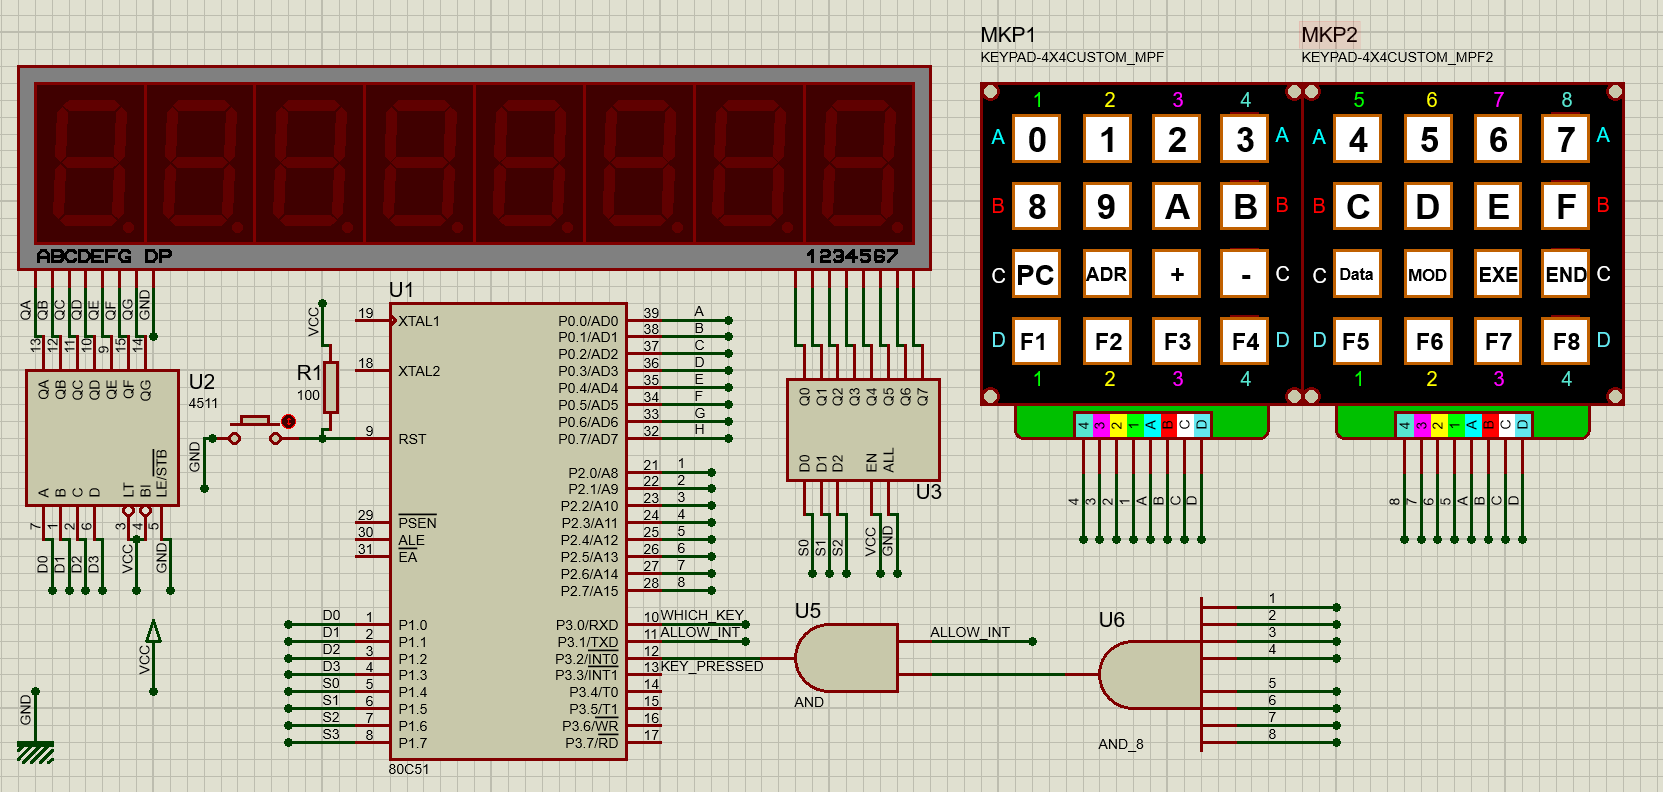
\includegraphics[width=6.625in, height=4in]{../Others/MAIN_CIRCUIT2.PNG}}
\caption{نمای تامیم یافته از طراحی مدار}
\label{fig}
\end{figure}
مشکلی که در این حالت به وجود می آید این است که در صورت نیاز به استفاده از حافظه خارجی با \underline{کمبود پورت روبه رو هستیم} که برای رفع آن میتوان ساختار کلید ها را به استفاده از 2 BDL کنترل کرد که در نتیجه تنها نیاز به استفاده از 8 پورت بود.
\\
\\
\clearpage
\problem{}
همانطور که گفته شد برای حل این مشکل میتوان 2 کار کرد راه معمول (که قرار است استفاده بکنیم) از $RAM$ برای ذخیره برنامه کاربر استفاده می کنیم.(در پایین به تفصیل آمده است) و یا اینکه یک محدوده برای کد اصلی برنامه تعیین کرد که کاربر توانایی نوشتن برنامه خود از آن آدرس به بعد را داشته باشد برای اجرای برنامه کاربر میتوانیم کل آن را به کل یک $subroutine$ نگاه کنیم و با ردن دکمه اجرا برنامه را به آدرس مشخص شروع برنامه کاربر $Call$ کنیم و قبل از این کار آخرین خانه برنامه کاربر را نیز با $Opcode$ مربوط به $RET$ پر بکنیم تا پس از اتمام برنامه کابر برنامه به روند خود بازگردد، مشخصا در هنگام اجرای برنامه کاربر روند برنامه اصلی مختل خواهد بود که قابل پیش بینی بود.
با پیاده سازی این روش (استفاده از حافظه استک برای به یاد داشتن نقطه قبلی اجرای برنامه) هیچ کدام از دستورات شرطی دچار مشکل نمی شود (تا زمانی که آدرس های شرطی وارد کد اصلی نشوند، که طبیعتا کاربر می بایست به آدرس دستورات برنامه خود $branch$ بزند و هزینه $branching$ به محدوده کد اصلی بر عهده کابر است (کاری که سیستم عامل میکند این است که در صورتی که برنامه های کاربردی اجازه دسترسی به حافظه مربوط به سیستم اصلی میکند یک $Exception$ تولید میکند ولی در اینجا برای این کار می بایست نحوه اجرای شرط ها را تغییر دهیم که به صرفه نیست) همچنین برای استفاده از دستور $Call$ نیز مشکلی به وجود نمی آید، تنها تفاوت این است که به جای شروع از خانه اول استک از خانه دوم استک برنامه آغاز خواهد شد. (که ساختاری بسیار سبک و مناسب است زیرا از سخت افزار خود میکروپروسسور استفاده میکند ولی با توجه به مشکلاتی که راجع به جدا بودن حافظه کد و برنامه به آن اشاره کردیم این موضوع در این میکروپروسسور نشدنی است).
\\
\\
اما روندی که قرار است اینجا پی بگیریم به این صورت است که چند خانه انتهایی حافظه (مثلا از $FF00H$ تا آخر) را برای حافظه مربوط به برنامه اصلی - مثلا اطلاعات مروبط به $7-segment$ که بحث آن شد و رجیستر های مجازی) استفاده می کنیم و بقیه حافظه 64 کیلوبایتی رم را برای استفاده برنامه کاربر مورد استفاده قرار دهیم. (بهتر است کاربر در برنامه خود از حافظه های اولیه استفاده نکند تا با کد برنامه خود در تلاقی نشود مثلا از آدرس های $1000H$ به بعد استفاده بکند)


با همان مکانیزمی که در قسمت قبل توضیح داده شد، محتویات خانه های حافظه رم پر میشود و در هر خانه حافظه $Op Code$ و یا $Operand$ قرار می گیرد (در مرحله وارد کردن داده).

حال یک جفت رجیستر از رجیستر ها را به عنوان $PC$ تعریف می کنیم و مقدار اولیه آن را صفر قرار می دهیم که به خانه اول رم اشاره بکند.

با زدن $EXE$ برنامه از آدرس صفر رم شروع به اجرا می شود به این صورت که ابتدا خانه اول حافظه رم خوانده می شود و متناسب با نوع دستور $Operand$ ها مربوطه در رجیستر ها لود می شوند (1 رجیستر برای $Opcode$ و حداکثر 3 تا برای $Operand$ ها) - مرحله $Fetch$ - و رجیستر $PC$ به یک خانه جلوتر می رود که $Opcode$ دستور بعدی است.

حال با توجه به محتویات مربوط به رجیستر $Opcode$ تصمیم میگیریم که باید چه کاری انجام دهیم - مرحله $Decode$ -، مثلا اگر خواست کاربر این بود که محتویات رجیستر $R6 $ را به $A$ منتقل کند این کار را با انتقال محتویات مربوط به رجیستر مجازی $R6 $ (که مثلا می تواند در آدرس $FF06H $ باشد) به رجیستر مجازی $A$ (که میتواند در آدرس $FF0AH$ باشد) انجام دهیم.
\\
دسته ای از دستورات هستند که روند خطی برنامه را مختل میکند و شاخه ایجاد میکنند دقیقا با همان ایده استفاده از پشته میتوان عملکرد این دستورات را شبیه سازی کرد، ضمنا از آن جایی که استک مستقل از کد اصلی است لازم نیست استک مجازی تعریف کنیم و چون در هنگام شبیه سازی برنامه نوشته شده توسط کاربر پروسسور نباید کاری بکند (میتواند همه وقفه ها را غیر فعال کند) می شود برای صرفه جویی از استک اصلی استفاده کرد و با هر دستور پرش یا $CALL$ محتویات رجیستر شبیه ساز $PC$ را وارد این استک کرد و در وقت لزوم آن را دوباره $pop$ کرد.
\\
\\
\underline{ممکن است مقادیر گفته شده در مورد آدرس ها در هنگام پیاده سازی (متناسب با شرایط) تغییر کند} 

\end{document}